%!xelatex = 'xelatex --halt-on-error %O %S'

\documentclass{thuemp}
\begin{document}

% 标题,作者
\emptitle{基于强化学习的无人机自主导航}
\empauthor{方桂安}{王涛老师}

% 奇数页页眉 % 请在这里写出第一作者以及论文题目
\fancyhead[CO]{{\footnotesize 方桂安: 无人系统导论课程设计}}


%%%%%%%%%%%%%%%%%%%%%%%%%%%%%%%%%%%%%%%%%%%%%%%%%%%%%%%%%%%%%%%%
% 关键词 摘要 首页脚注
%%%%%%%%关键词
\Keyword{机器学习, 强化学习, 无人机, 自主导航, 路径规划}
\twocolumn[
\begin{@twocolumnfalse}
\maketitle

%%%%%%%%摘要
\begin{empAbstract}
军事、运输、医疗和救援等许多领域都使用无人机作为下一代交通工具,其广泛应用于解决未知环境中的任务,但在这种情况下,我们无法事先获得环境的精确数学模型。本文提供了一个使用强化学习的框架,使无人机能够在这样的环境中自主导航。并对此进行了仿真和实验,以展示无人机如何成功地学会在未知环境中导航。还讨论了将强化学习算法应用于无人机系统和多无人机在线路径规划。这将有助于在更重要的应用中使用具有学习能力的无人机进行持续研究,例如野火监测、搜索和救援任务。
\end{empAbstract}

%%%%%%%%首页角注,依次为实验时间、报告时间、学号、email
\empfirstfoot{2021-12-17}{2021-01-10}{20354027}{fanggan@mail2.sysu.edu.cn}
\end{@twocolumnfalse}
]
%%%%%%%%!首页角注可能与正文重叠,请通过调整正文中第一页的\enlargethispage{-3.3cm}位置手动校准正文底部位置:
%%%%%%%%%%%%%%%%%%%%%%%%%%%%%%%%%%%%%%%%%%%%%%%%%%%%%%%%%%%%%%%%
%  正文由此开始
\wuhao 
%  分栏开始

\section{引~~言}
在涉及未知环境导航的任务中,如野火监测、目标跟踪或搜索救援,使用无人驾驶飞行器(无人机)正变得越来越普遍,因为它们可以搭载各种传感器,以相对较低的运行成本和较高的灵活性来测量环境。

但问题是,大多数当前的研究依赖于描述目标模型的准确性。然而,在大多数现实情况中很难做到这一点,因为关于目标环境的数据通常是有限的。

使用强化学习(RL)是克服这个问题的好方法,因为它允许无人机或无人机系统在没有环境模型的情况下学习和自主导航以适应不断变化的环境。


\section{项目可行性分析}
\enlargethispage{-3.3cm}
本课程的第三讲中我们学习了无人机系统概论,无人机系统的典型特征就是“平台无人,系统有人”,其导航方法通常分为自主导航、非自主导航两大类。

自主导航系统是指运动体完全依靠所载的设备自主地完成导航任务,和外界不发生任何光电联系。
非自主式导航系统是指机载设备需要依靠外部基准(地面基准或卫星基准)导航台来获取导航信息和数据的一种导航方式。

本项目由以下两点出发,探讨基于强化学习的无人机自主导航的可行性与需求性。


\subsection{设计思想来源}
复杂环境下无人机的自主导航控制系统是一个非常有研究意义和应用价值的挑战性课题, 它将无人系统的各个方面综合到一起, 包括传感器系统以及执行机构, 并且需要用于规划或者解决动态问题的额外计算能力。如何能够在未知复杂环境下进行行为控制决策, 具有对环境的自适应性和鲁棒性是无人机的自主导航控制系统所要解决的关键性问题。


由于无人飞行器的动力学特性非常复杂, 准确获取真实动力学参数难度很大, 特定模型参数的变化特征以及对于速度和航向控制的人类操控员经验的可获取性, 这些因素推动了基于模糊逻辑方法在导航控制规律研究中的应用。然而, 单纯依赖于人类感知和经验会导致一些严重的问题, 此外模糊逻辑系统尚存在其它的问题:1) 结构辨识问题;2) 维数灾难问题;3) 系统的模糊模型难以理解, 没有通用的分析工具来检验模糊系统的性能, 如动态特性、可控性以及稳定性等。而最早由Sutton教授提出的强化学习方法, 由于它是一种动作与环境的交互作用模式, 不依赖于环境模型、无需先验知识, 具有较强的自适应能力和鲁棒性等优点,因此结合强化学习的机器人导航控制方法研究已经引起越来越多研究人员的兴趣。其中Watkins在1989年提出的Q学习算法是一种最重要的强化学习方法, Q学习算法简单易实现, 并且其收敛性已经得到严格的证明\cite{一种基于强化学习的自主导航控制算法研究}。


本学期我们同时学习了无人系统导论和机器学习两门课程,且在大一我在参与大创项目后就进行了pytorch,tensorflow等深度学习框架的学习,另外去年我也完成了大学物理传感器的实验,并且作为智能科技协会的会长,我们有40台Tello无人机可供学生实验与研究。在调研并查阅相关论文资料之后,我决定结合这两门课所学的知识,尝试使用强化学习来协助无人机进行自主导航和路径规划。

\subsection{背景需求分析}
无人机按照应用领域可分为军用,民用两大类。

现代军用无人机被广泛用于执行军事电子侦察,电子对抗、预警、远距离攻击,战斗评估、军事地形航拍及测绘、反恐等方面。在减少参战人员伤亡,降低装备使用成本的同时,应对复杂的作战环境的能力,综合提高整体作战效率等方面都取得了不小成绩,军用无人机这些突出的使用特点正逐步受到各国军事部门的重视。无人机的身影已不仅限于出现在欧美科幻题材影片之中,在未来战场上多功能无人机的运用将出神入化、登峰造极,将发挥其决定战争胜败的关键作用。目前,为适应新军事革命时代潮流,维护国家主权及领土完整,维护和促进世界和平发展,拥有和发展自己的军事航空力量是我军的当务之急。我国国土幅员辽阔,边境海防线长,面对复杂的周边国际环境,研制先进的无人机来巩固和加强国防航空作战力量迫在眉睫。\cite{我国军用无人机发展趋势及现状分析}

近年来,民用无人机的市场发展迅速,业务范围不断拓展,为传统作业带了新的活力,使得娱乐体验更加多元化和震撼,在这种情况下,关于无人机相技术的研究也在逐渐增多,其中,感知避让(SAA)技术是民用无人机安全运行的重要保障,是安全有序融入国家空域系统的前提,避让算法使得无人机在没用户输入的情况下自主地规避障碍,是无人机自主飞行的基础。然而,现有研究大都针对特定问题,目前还很少有对自主导航本身知识结构的研究,而且普遍没有充分考虑到民用无人机实际任务作业的特点。\cite{李竺袁民用无人机自主飞行避让算法研究}


\section{总体架构设想}
\subsection{问题的定义}
假设我们有一个封闭的环境,其中关于它的先验信息是有限的。我们希望无人机从任意位置开始到达预先向机器人描述的目标(图1).
\begin{figure}[H]
\centering
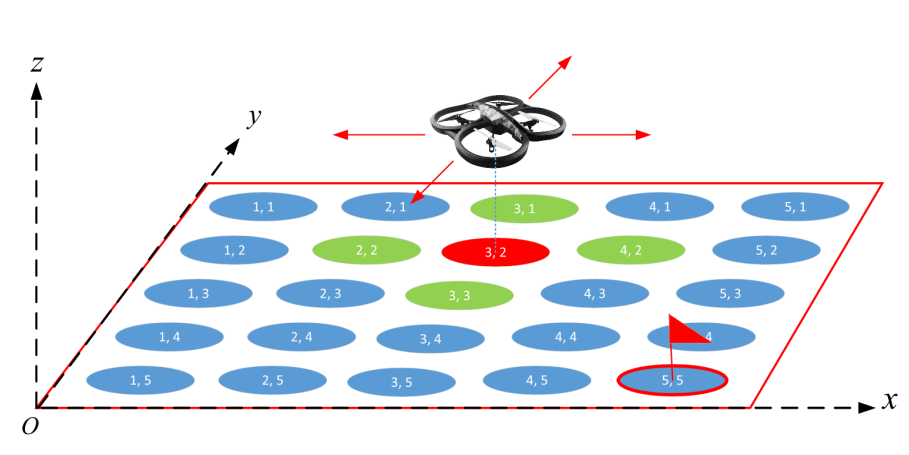
\includegraphics[width=0.8\linewidth]{./image/fig (1).png}
\caption{无人机在封闭环境中航行,状态空间离散,用离散的圆圈表示。红色圆圈是无人机的当前状态,绿色圆圈是无人机在下一次迭代中可以选择的选项,目标用红旗标记。} \label{fig:1}
\end{figure}
我们假设在任何位置,无人机都能观察到它的状态,即它的位置。如果我们有关于环境的全部信息,例如,到目标的确切距离或障碍物的位置,就可以根据环境的模型来构建无人机的运动规划,这样问题就变得简单了。然而,在更多的实际情况下,由于对环境的了解不够,建立精确的模型是不可能实现的。由于RL算法可以只依靠直接从系统中获得的数据,所以能很好地协助自主导航。在学习过程中,无人机需要将它所面临的情况映射到适当的行动上,以便使衡量无人机性能的数字信号(称为奖励)最大化。

为了执行给定的任务,无人机必须有一个学习组件,使其能够以最佳方式找到到达目标的方法。基于其当前状态sk(即无人机的位置)及其学习模型,无人机决定其希望达到的下一个状态sk+1的行动。然后,期望的位置将被作为位置控制器的输入,该控制器计算控制输入u(t)连接到下一层螺旋桨控制器。这个控制器将控制无人机的马达来发电,产生推力将其驱动至所需位置。另外,位置控制器必须能够克服无人机系统复杂的非线性动力学,实现无人机飞行时的稳定轨迹,以及在新状态下的悬停。图2展示了控制器流程框图。
\begin{figure}[H]
\centering
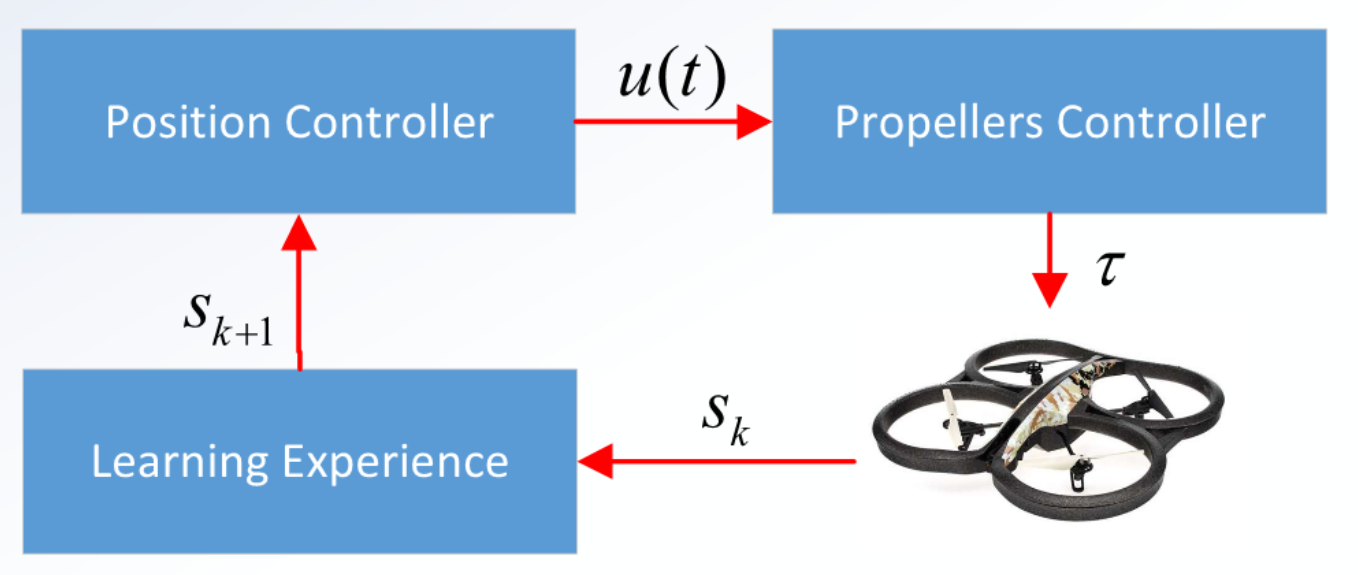
\includegraphics[width=0.8\linewidth]{./image/fig (2).png}
\caption{控制器流程框图} \label{fig:2}
\end{figure}
\subsection{强化学习与Q-learning}
基于RL的无人机-环境交互模型如图三所示,无人机通过与周遭环境的交互积累经验。
假设无人机下一个状态和奖励只取决于当前状态。
\begin{figure}[H]
\centering
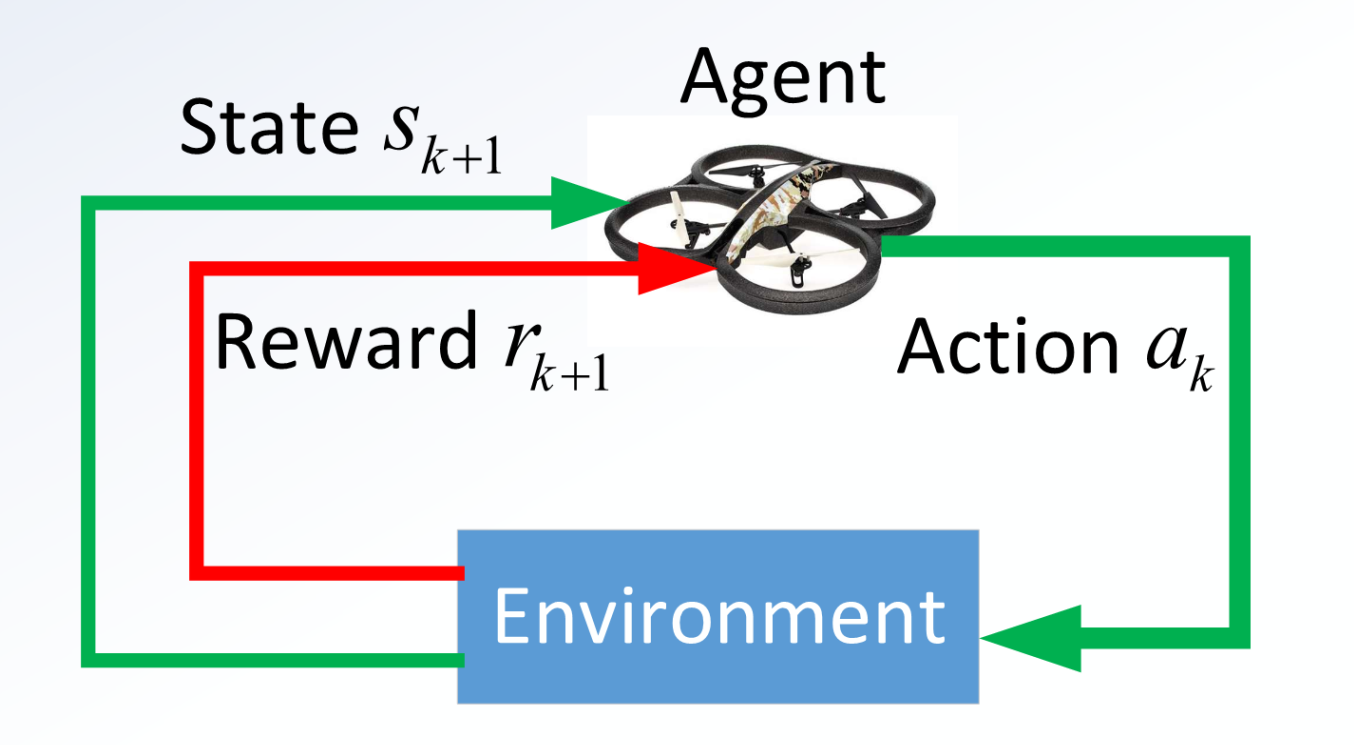
\includegraphics[width=0.8\linewidth]{./image/fig (3).png}
\caption{强化学习模型} \label{fig:3}
\end{figure}

模型可以概括为元组< S,A,T,R >,其中:
\begin{itemize}
\item S是一个有限的状态空间, $ s_{k} \in S $ 是无人机在步骤k时的状态。
\item A是一个有限的行动集合,$ a_{k} \in A $ 是无人机在步骤k采取的行动。
\item T是转移概率函数, $  S \times A \times   S \rightarrow[0,1] $ , 是无人机采取行动ak能从状态sk转移到状态sk+1的概率。我们假定 $ T\left(s_{k}, a_{k}, s_{k+1}\right)=1 $
\item R是奖励函数, $ S \times A \rightarrow \mathbb{R} $ 定义了无人机采取行动ak从状态sk转移到状态sk+1的即时奖励,即为 $ R\left(s_{k}, a_{k}\right)=r_{k+1} $。
\end{itemize}
无人机的目标是根据其状态制定一个行动方案使其到达终点时获得的奖励最大化。
在每个状态下,使用一个状态-行动评价函数Q(sk; ak)来量化在给定状态下选择一个
行动的收益,以用来协助无人机确定采取何种行动。无人机可以反复计算这个函数的
最优值,并从中得出一个最优行动方案。在本次作业中,我了解了一种流行的RL算法
:Q-learning\cite{1992Q}。计算出最优价值函数,并将其记录到数据库中,称为Q
表。这些数据可以被调用,以决定它采取何种行动来优化它在学习过程中的奖励。
对于每一次迭代,对最佳的状态-行动评价函数按照Bellman方程进行更新:
\begin{equation}\label{EQ1}
\begin{aligned}
Q_{k+1}\left(s_{k}, a_{k}\right) & \leftarrow(1-\alpha) Q_{k}\left(s_{k}, a_{k}\right) \\
&+\alpha\left[r_{k+1}+\gamma \max _{a \prime} Q_{k}\left(s_{k+1}, a \prime\right)\right]
\end{aligned}
\end{equation}

对于强化学习中的Exploration \& Exploitation 问题(探索-利用困境),采取 $ \epsilon -greedy $ 策略:

\begin{equation}\label{EQ2}
\begin{aligned}
\pi(s)=\left\{\begin{array}{ll}
\text { a random action } a, & \text { with probability } \epsilon \\
a \in \underset{a \prime}{\arg \max } Q_{k}\left(s_{k}, a \prime\right), & \text { otherwise }
\end{array}\right.
\end{aligned}
\end{equation}


为了使用Q学习算法,必须为系统中的无人机定义一组状态S、动作A和奖励R。由于连续空间太大,无法保证算法的收敛性,在实践中,通常将这些集合近似表示为离散有限集合。在本次作业中,我把环境看作是一个有限的半径为d的球面集,它们的中心构成一个网格。球体的中心表示环境的离散位置,而半径d是与中心的误差偏差。假设无人机可以在任何未知环境生成这些球体。无人机的状态被定义为它们在环境中的大致位置, $ s_{k} \triangleq c=\left[x_{c}, y_{c}, z_{c}\right] \in S $ ,其中 $ x_{c}, y_{c}, z_{c} $ 是状态sk时的球心坐标
。为了简化问题,这里只考虑二维平面上的状态,即无人机保持高度不变,如图1所示,球体压缩成圆形, $ s_{k} =\left[x_{c}, y_{c}\right]  $ 。

在每种状态下,无人机可以从一组四个可能的动作A中采取一个动作ak:在保持相同高度的同时,沿横向向北、向西、向南或向东前进。行动决定后,无人机将选择一个位置与所选动作相对应的相邻圆,即sk+1。无人机可以获得的奖励取决于它是否已经达到预先描述的目标G,到达目标G时会得到最大的奖励。到达其他不是预期目标的地方则将导致惩罚(负面奖励):
\begin{equation}\label{EQ3}
r_{k+1}=\left\{\begin{array}{ll}
100, & \text { if } s_{k+1} \equiv G \\
-1, & \text { otherwise }
\end{array}\right.
\end{equation}

\subsection{控制器和算法}
定义pt是无人机的实时位置,则有以下的比例增益控制器:
\begin{equation}
    u(t)=K_{p}\left(p(t)-s_{k+1}\right)=K_{p} e(t)
\end{equation}
其中u(t)是控制输入,Kp是比例控制增益,e(t)是实时位置p(t)和期望位置sk+1之间的跟踪误差。由于四旋翼飞行器的非
线性动力学,当无人机从一种状态导航到另一种状态,会出现不稳定的情况。因此需要使用PID控制器\cite{2016Modern}
来克服这一点,以确保产生较好的稳定性。
\begin{equation}
    u(t)=K_{p} e(t)+K_{i} \int e(t) d t+K_{d} \frac{d e}{d t}
\end{equation}
\begin{figure}[H]
\centering
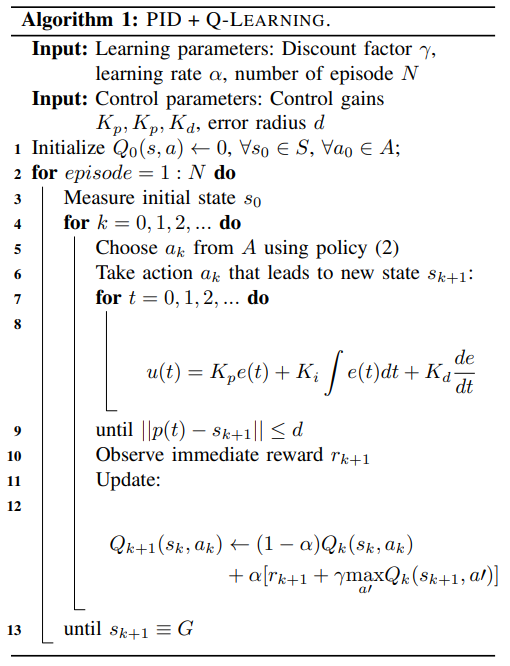
\includegraphics[width=1\linewidth]{./image/fig (5).png}
\caption{算法流程框图} \label{fig:2}
\end{figure}

\begin{figure}
    \centering
    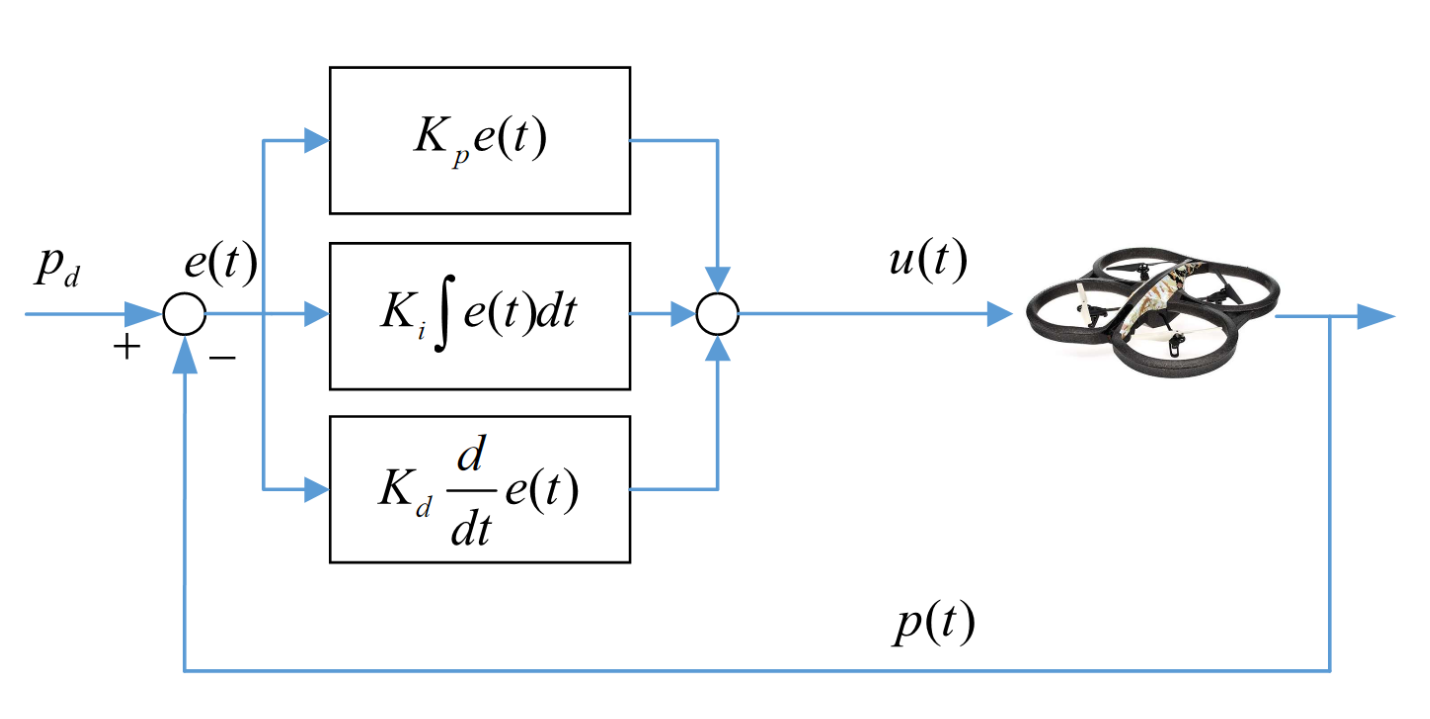
\includegraphics[width=0.8\linewidth]{./image/fig (4).png}
    \caption{PID控制器}
    \label{fig:my_label}
\end{figure}

\section{结论}
最终,我综合以上所述,在WSL2(Windows Subsystem for Linux)上结合ROS平台成功运行了仿真样例。虽然实现了基于 强化学习的无人机自主导航的基本功能,但仍存在许多问题。基于这些问题考虑的未来工作展望如下:
\begin{itemize}
    \item 无人机目前的性能仍有一定限制,运行此系统会造成CPU负载过高,耗电速率增大。应进一步优化系统流程,如考虑在应用启动后,仅在用户需要的时候唤醒摄像头等。
    \item 在引入神经网络后,自主导航算法在检测结果的表现上有了很大的提升,但其计算量也大大增加。复杂的计算需要消耗大量的资源,对无人机的性能有很大的影响。为了改善这一现状,考虑采用端云协同的分布式思想,由云端辅助无人机进行一部分的计算工作,让它们能更好地完成自主导航、路径规划。
    \item 未来,应该继续致力于在更重要的应用中使用具有学习能力的无人机,例如野火监测或搜索救援任务。该研究可以扩展到多智能体系统,以便多架无人机可以实时执行任务,其中学习能力可以帮助无人机在解决现实问题时具有更好的协调性和有效性。
\end{itemize}
%%%%%%%%%%%%%%%%%%%%%%%%%%%%%%%%%%%%%%%%%%%%%%%%%%%%%%%%%%%%%%%%
%  参考文献
%%%%%%%%%%%%%%%%%%%%%%%%%%%%%%%%%%%%%%%%%%%%%%%%%%%%%%%%%%%%%%%%
%  参考文献按GB/T 7714-2015《文后参考文献著录规则》的要求著录. 
%  参考文献在正文中的引用方法:\cite{bib文件条目的第一行}

\renewcommand\refname{\heiti\wuhao\centerline{参考文献}\global\def\refname{参考文献}}
\vskip 12pt

\let\OLDthebibliography\thebibliography
\renewcommand\thebibliography[1]{
  \OLDthebibliography{#1}
  \setlength{\parskip}{0pt}
  \setlength{\itemsep}{0pt plus 0.3ex}
}

{
\renewcommand{\baselinestretch}{0.9}
\liuhao
\bibliographystyle{gbt7714-numerical}
\bibliography{./TempExample}
}


\end{document}
